\begin{activite}[Lire un tableau]

Julie désire se rendre à Davos. Elle consulte les horaires des trains au départ d'Yverdon :

\begin{center}
\renewcommand*\tabularxcolumn[1]{>{\centering\arraybackslash}m{#1}}
 \begin{ttableau}{\linewidth}{7}
 \hline
 &  \cellcolor{F3} Train \newline n$^\circ$ 6\,123 & \cellcolor{F3} Train \newline n$^\circ$ 7\,258 & \cellcolor{F3} Train \newline n$^\circ$ 8\,766 & \cellcolor{F3} Train \newline n$^\circ$ 8\,989 & \cellcolor{F3} Train \newline n$^\circ$ 56\,789 & \cellcolor{F3} Train \newline n$^\circ$ 78\,995 \\
 \hline \cellcolor{F2} Yverdon & \cellcolor{Gris1} & 15 h 32 min & 16 h 05 min & 17 h 09 min & 17 h 20 min & 18 h 24 min \\
 \hline \cellcolor{F2} Bienne & 14 h 09 min & 16 h 32 min & \cellcolor{Gris1} & 17 h 58 min & 18 h 10 min & \cellcolor{Gris1} \\
 \hline \cellcolor{F2} Zürich  & 14 h 35 min & \cellcolor{Gris1} & \cellcolor{Gris1} & 18 h 11 min & 18 h 24 min & 19 h 18 min \\
 \hline \cellcolor{F2} Landquart & 14 h 58 min & \cellcolor{Gris1} & 17 h 32 min & \cellcolor{Gris1} & 18 h 47 min & \cellcolor{Gris1} \\
 \hline \cellcolor{F2} Davos & \cellcolor{Gris1} & 19 h 32 min & 20 h 15 min & 21 h 11 min & 21 h 32 min & 22 h 15 min \\
 \hline
 \end{ttableau}
 \end{center}

\vspace{1em}

\begin{partie}
Pourquoi certaines cases sont‑elles grisées ?
\end{partie}

\begin{partie}
Quel train est le plus rapide pour relier Yverdon à Davos ?
\end{partie}

\begin{partie}
En faisant une partie du trajet en voiture, Julie n'a passé que trois heures en train pour aller à Davos. De quelle(s) ville(s) a‑t‑elle bien pu partir ?
\end{partie}

\end{activite}

%%%%%%%%%%%%%%%%%%%%%%%%%%%%%%%%%%%%%%%%%%%%%%%%%%%%%%%%%%%%%%%%%%%%%%%%%

\begin{activite}[Utiliser des graphiques et des tableaux]

Pour déterminer quelques distances de freinage d'un véhicule sur route sèche, on a effectué des mesures à différentes vitesses, illustrées par le graphique ci-dessous :
\begin{center} 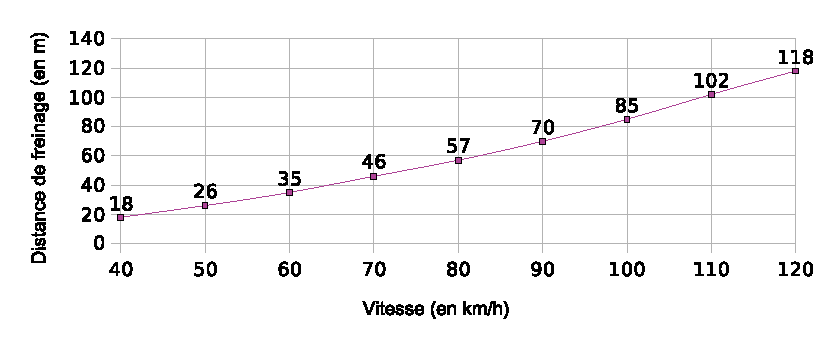
\includegraphics[width=14cm]{graph_freinage} \end{center}

\begin{partie}
Recopie et complète le tableau en utilisant le graphique :
\begin{center}
 \renewcommand*\tabularxcolumn[1]{>{\centering\arraybackslash}m{#1}}
 \begin{Ctableau}{\linewidth}{7}{c}
 \hline
 Vitesse (en km/h) & 50 & 70 & & & 110 & 120 \\\hline
 Distance de freinage (en m) & & & 70 & 85 & & \\\hline
  \end{Ctableau}
 \end{center}
\end{partie}

\vspace{1em}

\begin{partie}
Sur route mouillée, cette distance de freinage est deux fois plus grande que sur route sèche à vitesse égale.

Recopie et complète le tableau à double entrée suivant :
\begin{center}
 \renewcommand*\tabularxcolumn[1]{>{\centering\arraybackslash}m{#1}}
 \begin{Ctableau}{\linewidth}{4}{c}
 \hline
 Vitesse (en km/h) & 70 & & \\\hline
 Distance de freinage sur route sèche (en m) & & 35 &  \\\hline
 Distance de freinage sur route mouillée (en m) & & & 140 \\\hline
  \end{Ctableau}
 \end{center}
\end{partie}

\vspace{1em}

\begin{partie}
Aujourd'hui il pleut, et Joël part pour un petit tour de voiture en ville.

S'il doit s'arrêter pour éviter un obstacle, combien de mètres fera‑t‑il au maximum avant l'arrêt de son véhicule, s'il roule à la vitesse de 50 km/h.
\end{partie}

\end{activite}

%%%%%%%%%%%%%%%%%%%%%%%%%%%%%%%%%%%%%%%%%%%%%%%%%%%%%%%%%%%%%%%%%%%%%%%%%

\begin{activite}[Regrouper des données dans un tableau]

Dans un village, on a demandé aux familles le nombre d'enfants qu'elles avaient à charge. Le tableau ci‑dessous donne les réponses de chaque foyer.
\begin{center} 2 ; 3 ; 0 ; 1 ; 0 ; 1 ; 4 ; 2 ; 2 ; 0 ; 1 ; 6 ; 2 ; 3 ; 0 ; 7 ; 1 ; 0 ; 3 ; 2 ; 1 ; 3 ; 1 ; 3 ; 1 ; 1 ; 0 ; 7 ; 2 \end{center}

\begin{partie}
Recopie et complète le tableau suivant :
\begin{center}
\begin{tabularx}{\linewidth}{|c|*{10}{>{\centering \arraybackslash}X|}}
\hline \cellcolor{J1} Nombre d'enfants & 0 & 1 & 2 & 3 & 4 & 5 & 6 & 7 & Total \\
\hline \cellcolor{J2} Nombre de familles & & & & & & & & & \\
\hline
\end{tabularx} \\
\end{center}
\end{partie}

\vspace{1em}

\begin{partie}
Combien de familles ont quatre enfants ? \textbf{Moins de} trois enfants ? Combien de familles ont \textbf{exactement} quatre enfants ?
\end{partie}

\begin{partie}
Combien de familles ont \textbf{au moins} deux enfants ? \textbf{Plus de} quatre enfants ? \textbf{Au plus} quatre enfants ?
\end{partie}

\end{activite}

%%%%%%%%%%%%%%%%%%%%%%%%%%%%%%%%%%%%%%%%%%%%%%%%%%%%%%%%%%%%%%%%%%%%%%%%%

\begin{activite}[Utiliser un tableur]

\begin{partie}[À la cantine]
L'intendante du collège \emph{Rivegauche} a relevé le nombre de fois où chaque élève demi‑pensionnaire de sixième mange à la cantine durant la semaine et elle a reporté les résultats dans un tableau.
\begin{enumerate}
 \item Recopie son tableau dans une feuille de calcul en suivant ce modèle :
 \begin{center}
\begin{tabularx}{\linewidth}{|c|c|X|X|X|X|X|X|}
\hline \rowcolor{Gris1} & A & B & C & D & E & F & G \\
\hline \cellcolor{Gris1} 1 & & 1 jour & 2 jours & 3 jours & 4 jours & 5 jours & \\
\hline \cellcolor{Gris1} 2 & \cellcolor{G3} Nombre d'élèves & \cellcolor{J1} 20 & 33 & 21 & 47 & 37 & \cellcolor{B3} \\
\hline
\end{tabularx} \\
\end{center}
\vspace{.5em}
 \item Comment pourrais-tu nommer la cellule orange ? La verte ? La rose ?
 \item Combien de repas ont été servis à la cantine durant la semaine ? \label{TabsGraphsActi}
 \item Le tableur est capable de reproduire ce calcul si l'on saisit une formule dans la cellule $G2$. Une formule commence toujours par le signe «\,=\,». 
  \begin{itemize}
   \item Place le curseur dans la cellule $G2$ puis saisis la formule : « $= B2 + C2 + D2 + E2 + F2$ ». Appuie sur la touche «\,Entrée\,» du clavier. 
   \item Obtiens‑tu le même résultat qu'à la question \ref{TabsGraphsActi} ?
   \end{itemize}
 \item C'est le repas de Noël au collège ! Marc, Sonia et Sam, trois externes, désirent rejoindre leurs amis pour l'occasion. Modifie une cellule pour faire apparaître le changement d'effectif. Que remarques‑tu pour la cellule $G2$ ?
 \end{enumerate}
\end{partie}

\begin{partie}[Que de livres !]
En novembre 2009, l'imprimerie Volléro produit 2\,100 livres. Le directeur décide d'augmenter la production de 220 livres chaque mois dès le mois de décembre.
\begin{enumerate}
 \item Recopie le tableau suivant dans une feuille de calcul :
 \begin{center}
\begin{tabularx}{1.05\linewidth}{|c|*{6}{>{\centering \arraybackslash}X|}}
\hline \rowcolor{Gris1} & A & B & C & D & E \\
\hline \cellcolor{Gris1} 1 & \cellcolor{G3} Mois & \small{Novembre} 2009 & \small{Décembre} 2009 & \small{Janvier} 2010 & \small{Février} 2010
 \\
\hline \cellcolor{Gris1} 2 & \cellcolor{G2} Nombre de livres & 2\,100 & & & \\
\hline
\end{tabularx} \\
\end{center}
\vspace{0.5cm}         
 \item Saisis les formules permettant de compléter le tableau.
 \item Comment ferais‑tu pour calculer le nombre de livres produits en mars 2010 ?
 
Le tableur peut reproduire cette méthode en saisissant une formule dans la cellule $F2$.
 \item Place le curseur dans la cellule $F2$ et saisis la formule : « $= E2 + 220$ ». Comment comprends‑tu cette formule ?
 \item Quelle serait la formule à saisir en $G2$ pour calculer le nombre de livres produits en avril 2010 ? \label{Tabs&Graphs_acti2}
 \item Copie le contenu de la cellule $F2$ et colle‑le dans la cellule $G2$. Tu peux voir le résultat sur la ligne située au-dessus de ta feuille de calcul. Que s'est‑il passé ?
\begin{center} 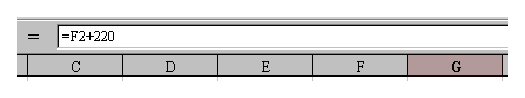
\includegraphics[width=11.2cm]{feuille_calcul} \end{center}
 \item Le directeur aimerait savoir quand (mois et année) son usine produira plus de 8\,000 livres par mois. En répétant plusieurs fois la méthode de la question \ref{Tabs&Graphs_acti2}, réponds à la question du directeur.
 \end{enumerate}
\end{partie}


\end{activite}

%%%%%%%%%%%%%%%%%%%%%%%%%%%%%%%%%%%%%%%%%%%%%%%%%%%%%%%%%%%%%%%%%%%%%%%%%